\section{Combined System} \label{sec:TotalSystem}
This appendix will describe the total system, shown on \autoref{fig:totalSystem}, which is the combination of the ANC system shown on \autoref{fig:SimulinkANC} and the predictor shown on \autoref{Fig:PredictionSimulink}. These are already described so they will not be described again. 
\begin{figure}[H]
	\centering
	\tikzsetnextfilename{Totalsystemoverview}
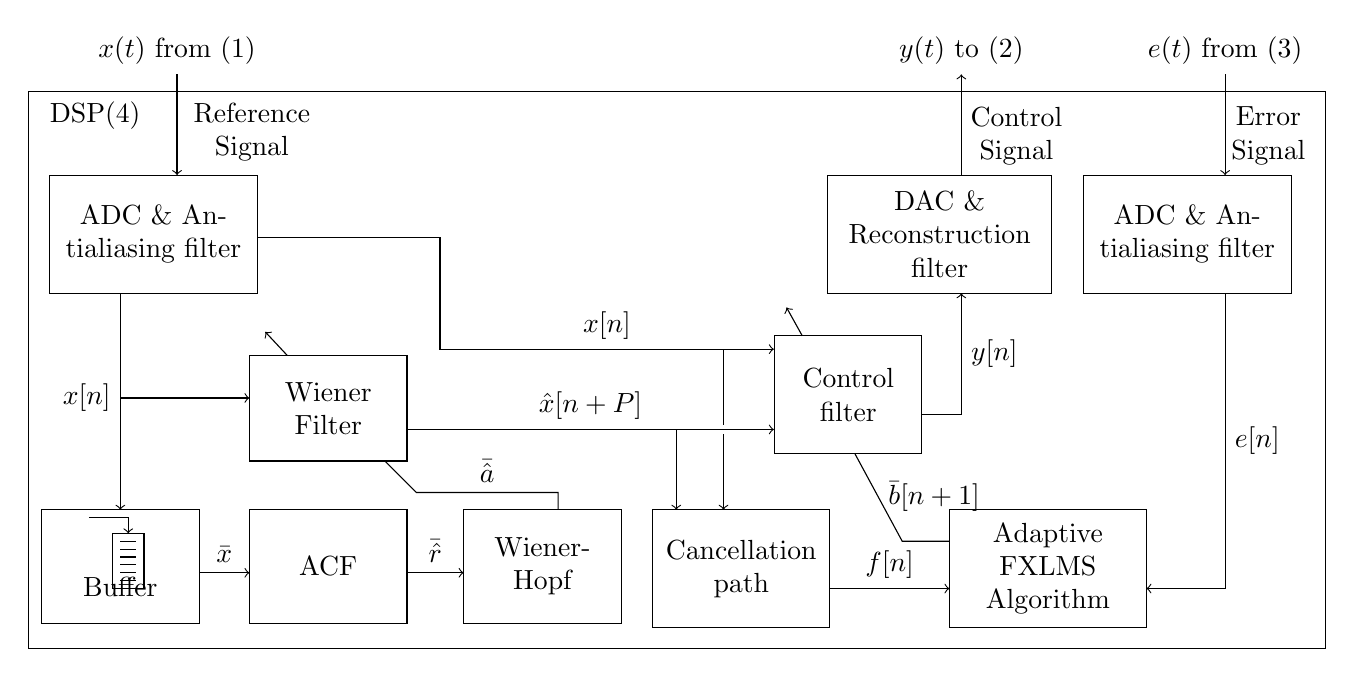
\begin{tikzpicture}
\draw  (-6.96,-2.17) rectangle node[text width=2.5cm,align=center] {ADC \& Antialiasing filter} (-4.32,-3.67);
\draw  (0.7,-6.42) rectangle node[text width=2.5cm,align=center] {Cancellation \\ path}(2.95,-7.92);
\draw  (4.47,-6.42) rectangle node[text width=2.5cm,align=center] {Adaptive FXLMS Algorithm} (6.97,-7.92);

\draw  (2.25,-4.21) rectangle node[text width=1.5cm,align=center,fill=white] {Control filter} (4.12,-5.71);
\draw  (2.92,-2.17) rectangle node[text width=2.5cm,align=center] {DAC \& \\ Reconstruction filter}(5.77,-3.67);
\draw  (6.17,-2.17) rectangle node[text width=2.5cm,align=center] {ADC \& Antialiasing filter}(8.81,-3.67);

\draw  (-7.23,-1.11) rectangle (9.25,-8.18);
\node at (-6.38,-1.41) {DSP(4)};
\node [text width=2cm,align=center] at (-4.39,-1.62) {Reference Signal};

\draw[->] (2.95,-7.42) -- node[above]{$f[n]$} (4.47,-7.42);

\draw[->] (7.97,-3.67) -- node[right]{$e[n]$} (7.97,-7.42)  -- (6.97,-7.42);

\draw [->](7.97,-0.89) node[above]{$e(t)$ from (3)} -- (7.97,-2.17) ;
\draw [->](4.62,-2.17)  --  (4.62,-0.89) node[above]{$y(t)$ to (2)};




\draw[->] (4.12,-5.21) -- (4.62,-5.21) --node[right]{$y[n]$} (4.62,-3.67);
\draw [->](-5.34,-0.89) node[above]{$x(t)$ from (1)} -- (-5.34,-2.17);
\node [text width=2cm,align=center] at (5.32,-1.67) {Control Signal};
\node [text width=1.5cm,align=center] at (8.52,-1.67) {Error Signal};

\draw (4.47,-6.82) -- (3.87,-6.82) --node[above=0.25,right]{$\bar{b}[n+1]$} (3.27,-5.71);
\draw [->](2.6,-4.21) -- (2.4,-3.85);


%% Boxes
\draw  (-4.42,-5.8) rectangle node[text width=2cm,align=center] {Wiener Filter}(-2.42,-4.46);
\draw  (-2.42,-6.42) rectangle node[text width=2cm,align=center] {ACF}(-4.42,-7.86);
\draw  (-5.06,-6.42) rectangle node[text width=2cm,align=center,below=0.2] {Buffer}(-7.06,-7.86);
\draw  (-1.7,-6.42) rectangle node[text width=1.5cm,align=center] {Wiener- Hopf}(0.3,-7.86);



%%Buffer
\draw (-5.76,-7.42) node (v1) {} -- (-6.16,-7.42) -- (-6.16,-6.72) -- (-5.76,-6.72) -- (-5.76,-7.42);
\draw (-6.06,-6.82) -- (-5.86,-6.82);
\draw (-6.06,-6.92) -- (-5.86,-6.92);
\draw (-6.06,-7.02) -- (-5.86,-7.02);
\draw (-6.06,-7.12) -- (-5.86,-7.12);
\draw (-6.06,-7.22) -- (-5.86,-7.22);
\draw (-6.06,-7.32) -- (-5.86,-7.32);
\draw [->](-6.46,-6.52) -- (-5.96,-6.52) -- (-5.96,-6.72);


%% Lines
\draw [->](-5.06,-7.22) -- node[above]{$\bar{x}$} (-4.42,-7.22);
\draw [->](-2.42,-7.22) -- node[above]{$\bar{\hat{r}}$}(-1.7,-7.22);
\draw (-0.5,-6.42) -- (-0.5,-6.2) -- node[above]{$\bar{\hat{a}}$} (-2.3,-6.2) -- (-2.7,-5.8);


\draw [->](-3.94,-4.46) -- (-4.22,-4.16);
\draw [->](-6.06,-5)  node[left]{$x[n]$} -- (-4.42,-5);
\draw [->](-6.06,-3.68) -- (-6.06,-6.42);
\draw [->](-2.42,-5.4) --  node[above]{$\hat{x}[n+P]$}(2.24,-5.4);

\draw [->](-4.32,-2.96) -- (-4.06,-2.96) -- (-2,-2.96) -- (-2,-4.38) -- node[above]{$x[n]$} (2.24,-4.38);
\draw (1.6,-4.38) -- (1.6,-5.34);
\draw [->](1.6,-5.46) -- (1.6,-6.42);
\draw [->](1,-5.4) -- (1,-6.42);
\end{tikzpicture}
	\caption{Total ANC system. }
	\label{fig:totalSystem}
\end{figure}

The system shown on \autoref{fig:totalSystem} utilize both the predicted input $\hat{x}[n]$ and the measured input $x[n]$, in the control filter and CP. This expands \autoref{eq:Outputapp} to \autoref{eq:ControlExpandedapp} and \autoref{eq:CPapp} to \autoref{eq:CPExpandedapp}.
\begin{equation}\label{eq:Outputapp}
y[n]=\sum_{j=0}^{L-1}b_j[n]x[n-j]
\end{equation}
\begin{equation}\label{eq:CPapp}
f[n]=\sum_{j=0}^{L-1}c_jx[n-j]
\end{equation}
\begin{equation}\label{eq:ControlExpandedapp}
y[n+P]=\sum^{P-1}_{j=0}b_j[n]\hat{x}[(n+P)-j]+\sum^{L-1}_{j=P}b_j[n]x[(n+P)-j]
\end{equation}

\begin{equation}\label{eq:CPExpandedapp}
f[n+P]=\sum^{P-1}_{j=0}c_j\hat{x}[(n+P)-j]+\sum^{L-1}_{j=P}c_jx[(n+P)-j]
\end{equation}

No other changes has been made to the total system and it is the system which will be used for simulation.

\newpage
\section{Simulink Combined System Test} \label{sec:SimulinkTotalSystem}

\subsection{Description}
This appendix will simulate the ANC system, shown on \autoref{fig:totalSystem}, which is a combination of the ANC system show on \autoref{fig:SimulinkANC} and the predictor shown on \autoref{Fig:PredictionSimulink}. The simulation will test if the combined LP FXLMS system is dependent on delays if the same delay is predicted by the predictor. All functions for the ANC system and predictor are already described in \autoref{sec:ANCSimulation} and \autoref{sec:predicSimulink} respectively. The "real world" simulink system is shown on \autoref{fig:SimulinkRealWorld}.

\subsection{Diagram}
\begin{figure}[H]
	\centering
	\includegraphics[width=1\textwidth]{figures/GrandTest/TotalSystem}
	\caption{Total ANC system in Simulink.}
	\label{fig:SimulinktotalSystem}
\end{figure}


\subsection{Variables}
\begin{lstlisting} [language=MATLAB, caption=Variables]
N 			= 1200; 		%is the frame length 
overlap 	= 1100;			%is the overlap in the buffer "O"
prediction 	= 10; 			%is how far the algorithm should predict "P"
fs 			= 48000; 		%is the sample frequency of the input signal 
w           = hamming(N)	% could be replaced by other window functions
M           = N;			% is equal to N in all cases
L  			= 960;  	 	%is the length of the filter
HPCoef;  		 			%is the coeffiecients for the measured HP
CPCoef;  		 			%is the coeffiecients for the measured CP
u  			= 0.001;		%is the convergence factor
delay 			 			%is the delay of the ADC delay and DAC delay
\end{lstlisting}

\subsection{Functions}

\begin{lstlisting} [language=MATLAB, caption=Simulink Expanded control filter function., label=Lst:controlFilterExpandedReal]
function y = fcn(xhat,x,b,L,prediction)

%Setup of interal variables
persistent xIn;     %buffer for input

if isempty(xIn)
  xIn=zeros(1,L);
end

xIn = [xhat xIn(1:prediction-1) x xIn(prediction+1:end-1)];

% FIR filter
y = xIn*b;
\end{lstlisting}

\begin{lstlisting} [language=MATLAB, caption=Simulink Expanded CP function., label=Lst:cpExpandedReal]
function y  = fcn(x,xhat,CPCoef,L,prediction)

%Setup of interal variables
persistent xIn;     %buffer for input

%Setup of internal variables if the variables are not defined
if isempty(xIn)
  xIn=zeros(1,L);
end

%buffer for input
xIn = [xhat xIn(1:prediction-1) x xIn(prediction+1:end-1)];

y = xIn*CPCoef;
\end{lstlisting}

\subsection{Test}
A simulation of the total system with different ADC and DAC delay is to be made to see if delays affect the attenuation of the system. The delays are varied from 2 to 50 in steps of 2. For each simulation the RMS of the output is compared to the RMS of the input filtered with the HP transfer function using \autoref{eq:testANC2}. 

\begin{equation}\label{eq:testANC2}
	Attenuation=20 \cdot log_{10} \left (\frac{\sqrt{\sum\limits_{i=1}^{N}HPSig^2[n-i]}}{\sqrt{\sum\limits_{i=1}^{N}ANCsig^2[n-i]}}  \right )
\end{equation}

The combined algorithm is not simulated a delay 0, as the predictor would be redundant. All other results are shown on \autoref{fig:delayRatioTotal} together with the results of the system with no predictor described in \autoref{sec:ANCSimulation}.
\begin{figure}[H]
	\captionsetup[subfigure]{oneside,margin={1cm,-2cm}}
	\centering
		\hspace{-20mm}
	\begin{subfigure}[b]{0.40\textwidth}
	\centering
		\tikzsetnextfilename{delayTestTotal}	
		\input{figures/GrandTest/DelayRatioTotal.tex}
		\caption{ Attenuation of feedforward FXLMS (blue) compared with feedforward LP FXLMS (red) with different system delays. The blue line is identical to that in \autoref{Fig:delayRatioAppendix}}
		\label{fig:delayRatioTotal}
	\end{subfigure}
	\hspace{20mm}
	\begin{subfigure}[b]{0.40\textwidth}
	\centering
	\tikzsetnextfilename{ComparedConusmerHPOurAppendix}
	% This file was created by matlab2tikz.
%
%The latest updates can be retrieved from
%  http://www.mathworks.com/matlabcentral/fileexchange/22022-matlab2tikz-matlab2tikz
%where you can also make suggestions and rate matlab2tikz.
%

\definecolor{mycolor1}{rgb}{0.00000,0.44700,0.74100}%
\definecolor{mycolor2}{rgb}{0.85000,0.32500,0.09800}%
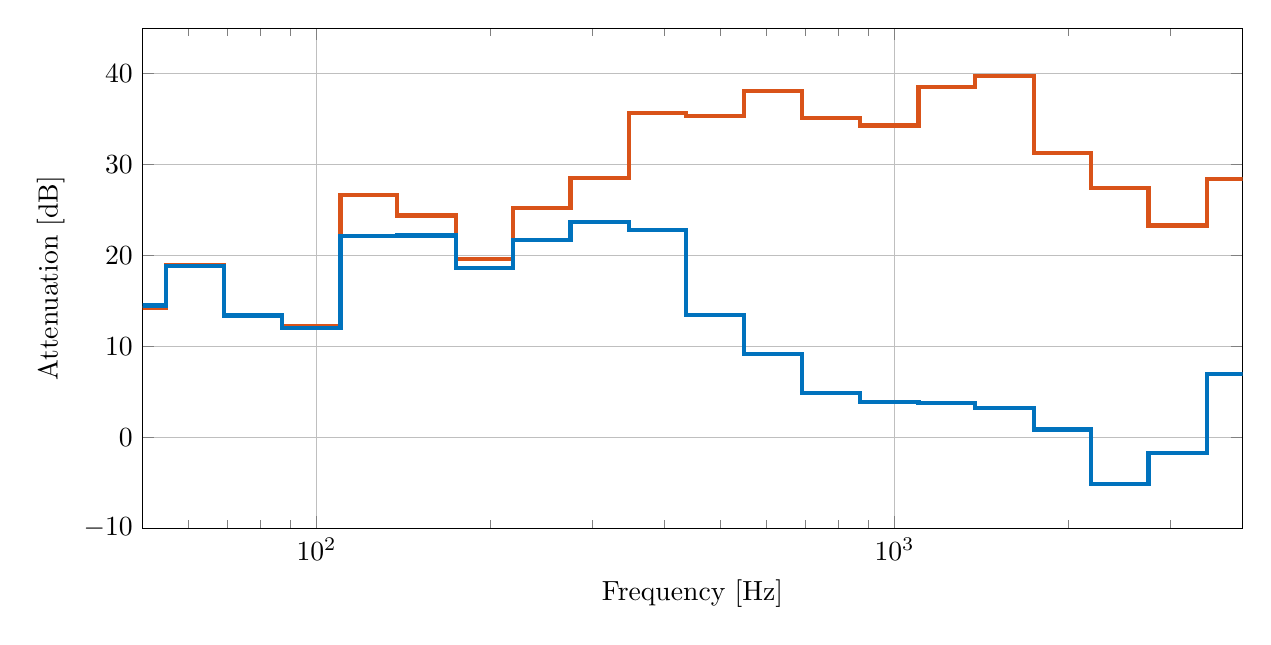
\begin{tikzpicture}

\begin{axis}[%
width=5.5in,
height=2.5in,
scale only axis,
%scaled y ticks = false,
xmode=log,
xmin=50,
xmax=4000,
xlabel={Frequency [Hz]},
xmajorgrids,
ymin=-10,
ymax=45,
ytick={-10,0,...,40},
ylabel={Attenuation [dB]},
ymajorgrids,
axis background/.style={fill=white},
title style={font=\bfseries},
%title={Comparison}
]
\addplot[const plot,color=mycolor2,solid,forget plot,thick, line width=1.5pt] plot table[row sep=crcr] {%
	21.9	8.53\\
	27.5	9.92\\
	34.7	15\\
	43.6	14.2\\
	54.9	19\\
	69.1	13.5\\
	87.1	12.2\\
	110	26.7\\
	138	24.4\\
	174	19.6\\
	219	25.2\\
	275	28.5\\
	347	35.7\\
	436	35.3\\
	549	38.1\\
	691	35.1\\
	871	34.3\\
	1.1e+03	38.5\\
	1.38e+03	39.7\\
	1.74e+03	31.3\\
	2.19e+03	27.4\\
	2.75e+03	23.3\\
	3.47e+03	28.4\\
	4.36e+03	24.1\\
	5.49e+03	13.9\\
	6.91e+03	10.2\\
	8.71e+03	23.6\\
	1.1e+04	19.1\\
	1.38e+04	13.2\\
	1.79e+04	2.94\\
};
\addplot[const plot,color=mycolor1,solid,forget plot,thick,line width=1.5pt] plot table[row sep=crcr] {%
	21.9	8.7\\
	27.5	10.1\\
	34.7	15.2\\
	43.6	14.5\\
	54.9	18.8\\
	69.1	13.4\\
	87.1	12\\
	110	22.1\\
	138	22.2\\
	174	18.6\\
	219	21.7\\
	275	23.7\\
	347	22.8\\
	436	13.5\\
	549	9.13\\
	691	4.85\\
	871	3.85\\
	1.1e+03	3.75\\
	1.38e+03	3.18\\
	1.74e+03	0.859\\
	2.19e+03	-5.09\\
	2.75e+03	-1.73\\
	3.47e+03	6.95\\
	4.36e+03	15.9\\
	5.49e+03	6.78\\
	6.91e+03	7.84\\
	8.71e+03	24.8\\
	1.1e+04	15\\
	1.38e+04	13.8\\
	1.79e+04	4.07\\
};
\end{axis}
\end{tikzpicture}%
	\caption{Frequency response of feedforward FXLMS (blue) compared with feedforward LP FXLMS (red). Results are filtered using a class 0 1/3 octave filter bank \cite{OctaveBand}.}
	\label{fig:ANCcompareALLAppendix}
	\end{subfigure}	
	\caption{Results of the simulation}	
\end{figure}



\subsection{Conclusion}
The combined Feedforward LP FXLMS algorithm increase the attenuation of speech compared to a feedforward FXLMS algorithm. 
